\documentclass{article}
\usepackage[utf8]{inputenc}

\usepackage{natbib}
\usepackage{graphicx}

\usepackage[slovene]{babel}
\usepackage{amsmath}
\usepackage{amsfonts}
\usepackage{amssymb}

\usepackage[T1]{fontenc}
\usepackage{listingsutf8}
\lstset{literate={č}{{\v c}}1 {š}{{\v s}}1 {ž}{{\v z}}1}
\lstset{basicstyle=\ttfamily, language=bash}

\usepackage{algorithm}
\usepackage{algorithmicx}
\usepackage{algpseudocode}

\usepackage{tikz}
\usetikzlibrary{graphs,quotes,arrows.meta}
\usetikzlibrary{positioning}


\title{3. domača naloga}
\author{Lovro Habjan}
\date{\today}


\begin{document}

\maketitle

\section{Problem 1}

\subsection{Podproblem A}

Napisati moramo algoritem, ki izračuna unijo dveh konveksnih ovojnic. To storimo
tako, da točke obeh ovojnic združimo in uporabimo algoritem
\textsc{Graham-Scan}, kot je opisan v \cite{cormen2009introduction}. Končna
psevdokoda je predstavljena z algoritmom \ref{alg-1a}.

\begin{algorithm}
	\caption{Unija konveksnih ovojnic}
	\label{alg-1a}

	\begin{algorithmic}[1]
		\Function{Convex-Hull-Union}{$Q_1$, $Q_2$}
			\State $Q := $ \Call{Concatenate}{$Q_1$, $Q_2$}
			\State \Return \Call{Graham-Scan}{$Q$}S
		\EndFunction

		\Statex

		\Function{Graham-Scan}{$Q$}
			\State $p_0$ je točka v $Q$ z najmanjšo koordinato $y$ ali najbolj
				leva točka v primeru večih takih točk
			\State $\langle p_1, p_2, ..., p_n \rangle$ ostale točke v $Q$
			\State $S := $ prazen sklad
			\State \Call{Push}{$p_0$, $S$}
			\State \Call{Push}{$p_1$, $S$}
			\State \Call{Push}{$p_2$, $S$}
			\For{$i = 3$ to $m$}
				\While{kot, ki ga tvorijo \Call{Next-To-Top}{$S$},
					\Call{Top}{$S$} in $p_i$ ne naredijo levega ovinka}
					\State \Call{Pop}{$S$}
				\EndWhile
				\State \Call{Push}{$p_i$}
			\EndFor
			\State \Return $S$
		\EndFunction
	\end{algorithmic}
\end{algorithm}


\subsection{Podproblem B}

Napisati moramo algoritem, ki preveri, če se konveksni ovojnici sekata. Za idejo
rešitve uporabimo Jordanov teorem, ki pravi, da povezana krivulja (ali v našem
primeru poligon) deli ravnino na dva dela. Točke lahko ležijo v poligonu ali
izven njega. Naša rešitev je sledeča - za vsako točko v konveksni ovojnici $Q_1$
preverimo, če leži znotraj konveksne ovojnice $Q_2$. Če obstaja vsaj ena taka
točka, se konveksni ovojnici $Q_1$ in $Q_2$ sekata. Da za točko preverimo, ali
leži v poligonu, iz nje narišemo neskončen trak v poljubni smeri. Če bo trak
sekal liho število daljic konveksne ovojnice, točka leži znotraj poligona, v
sodem primeru pa zunaj poligona.

Najprej preverimo, če je točka $p = (x, y) \in Q_1$ leži v konveksni ovojnici
$Q_2$. Nato iz $p$ potegnemo neskončen poltrak v smeri $d_p = (1, 0)$.
Parametriziran je kot
\begin{equation*}
	r(t_1) = p + d_p t_1 \text{  for}\ t_1 \in [0, \infty)
\end{equation*}
Daljica konveksne ovojnice je parametrizirana kot
\begin{equation*}
	q(t_2) = a + (b - a) t_2 \text{ for}\ t_2 \in [0, 1]
\end{equation*}
kjer sta $a$ in $b$ točki konveksne ovojnice $Q_2$.

Najprej preverimo, če sta poltrak in daljica vzporedni - takrat velja $d_p \times
(b - a) = 0$. V tem primeru preverimo, če točka $p$ leži na daljici.

Če poltrak in daljica nista vzporedni, izpeljemo enačbi za $t_1$ in $t_2$:
\begin{align*}
	r(t_1) &= q(t_2) \\
	p + d_p t_1 &= a + (b - a) t_2 \\
	(p + d_p t_1) \times (b - a) &= (a + (b - a) t_2) \times (b - a) \\
	p \times (b - a) + t_1 (d_p \times (b - a)) &= a \times (b - a) + t_2 ((b - a) \times (b - a)) \\
	t_1 (d_p \times (b - a)) &= (a - p) \times (b - a) \\
	t_1 &= \frac{(a - p) \times (b - a)}{d_p \times (b - a)}
\end{align*}

\begin{align*}
	p + d_p t_1 &= a + (b - a) t_2 \\
	(p + d_p t_1) \times d_p &= (a + (b - a) t_2) \times d_p \\
	p \times d_p + t_1 (d_p \times d_p) &= a \times d_p + t_2 ((b - a) \times d_p) \\
	t_2 ((b - a) \times d_p) &= (p - a) \times d_p \\
	t_2 &= \frac{(a - p) \times d_p}{d_p \times (b - a)}
\end{align*}

Če velja $t_1 \geq 0$ in $0 \leq t_2 \leq 1$, obstaja presečišče. Če vse točke
ležijo v znotraj ali zunaj konveksne ovojnice, se $Q_1$ in $Q_2$ ne sekata.

Psevdokoda je prikazana z algoritmom \ref{alg-1b}.

\begin{algorithm}
	\caption{Se dve konveksni ovojnici sekata}
	\label{alg-1b}

	\begin{algorithmic}[1]
		\Function{ConvexHull-Intersect?}{$Q_1$, $Q_2$}
			\State $d = (1, 0)$
			\State $segments$ so daljice, ki sestavljajo $Q_2$.
			\State $numInside := 0$
			\For{$p_i \in Q_1$}
				\If{$p_i \in Q_2$} \Return \textsc{True}
				\EndIf
				\State $numIntersections := 0$
				\State $lineVec = q_2 - q_1$
				\For{$(q_i, q_j) \in segments$}
					\If{$d \times lineVec == 0$}
						\If{$p$ leži na daljici} \Return \textsc{True}
						\EndIf
					\EndIf
					\State $t_1 = ((q_1 - p_i) \times lineVec) / (d \times lineVec)$
					\State $t_2 = ((q_1 - p_i) \times d) / (d \times lineVec)$
					\If{$t_1 \geq 0$ in $0 \leq t_2 \leq 1$}
						\State $numIntersections := numIntersections + 1$
					\EndIf
				\EndFor
				\If{$numIntersections$ \% $2 == 1$}
					\State $numInside := numInside + 1$
				\EndIf
			\EndFor
			\If{$numInside == 0$ || $numInside == \lvert Q_1 \rvert$}
				\State \Return \textsc{False}
			\Else
				\State \Return \textsc{True}
			\EndIf

		\EndFunction
	\end{algorithmic}
\end{algorithm}


\subsection{Podproblem C}

Algoritme smo implementirali v programskem jeziku Haskell.

Za algoritem \ref{alg-1a} smo za sklad uporabili seznam, ki je vgrajena
podatkovna struktura v programskem jeziku. Zaznavo levega ali desnega obrata
smo izračunali s pomočjo determinante, kot je opisano v
\cite{cormen2009introduction}.

Za algoritem \ref{alg-1b} smo dodali dodatno preverjanje, če gre poltrak skozi
določeno točko v $Q_2$, saj je bilo v takem primeru presek štet dvakrat.
Štetje števila točk znotraj ali zunaj je bilo implementirano z novim podatkovnim
tipom, s katerim smo skrbeli, da smo ob prvi priložnosti zaključili preverjanje
sekanja poltraka s segmenti.

Program smo testirali z nekaj testnimi primeri. Prvi testni primer je enak
podanemu testnemu primeru. Slika \ref{fig:test02} prikazuje drugi primer, kjer
imamo dve konveksni ovojnici, ki se ne sekata. Slika \ref{fig:test03} prikazuje
tretji primer, kjer se konveksni ovojnici sekata. Slika \ref{fig:test04}
prikazuje četrti primer, kjer ena konveksna ovojnica vsebuje drugo. Program vrne
naslednje rezultate za testne primere:

\begin{lstlisting}
$ ghc 1c.hs
[1 of 1] Compiling Main             ( 1c.hs, 1c.o )
Linking 1c ...
$ ./1c < test01.txt
4.0 5.0 4.0 2.0 0.0 0.0
-1.0 0.0 1.0 1.5 1.5 0.0
TRUE
$ ./1c < test02.txt
-4.0 1.95 6.0 4.0 -7.0 -10.0 -9.0
-4.0 -2.9 -1.0 3.2 3.0 0.0 -3.0
FALSE
$ ./1c < test03.txt
-1.0 2.0 5.0 6.0 4.0 1.0 -2.0
-1.0 -1.0 -1.0 1.0 3.0 3.0 1.0
TRUE
$ ./1c < test04.txt
0.0 4.0 5.0 1.0 -3.0 -3.0
-5.0 -4.0 -1.0 3.0 2.0 -2.0
FALSE
\end{lstlisting}

Izvorna koda se nahaja v datoteki \textit{1c.hs}.

\begin{figure}
	\centering
	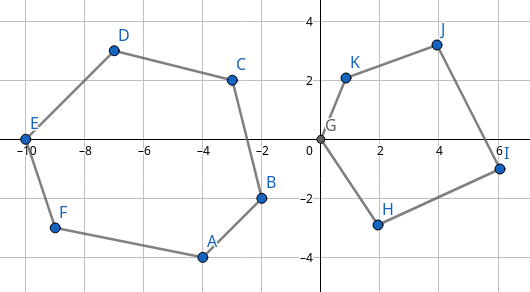
\includegraphics[scale=0.5]{./figs/test02.png}
	\caption{Konveksni ovojnici drugega testnega primera}
	\label{fig:test02}
\end{figure}

\begin{figure}
	\centering
	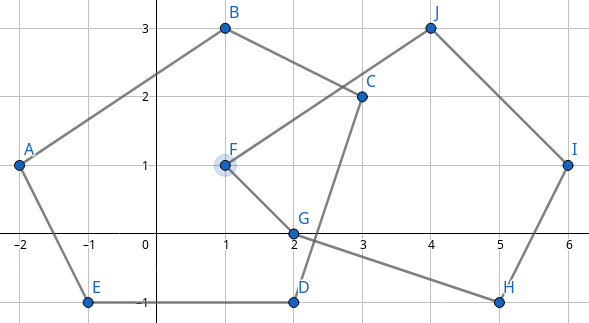
\includegraphics[scale=0.4]{./figs/test03.png}
	\caption{Konveksni ovojnici tretjega testnega primera}
	\label{fig:test03}
\end{figure}

\begin{figure}
	\centering
	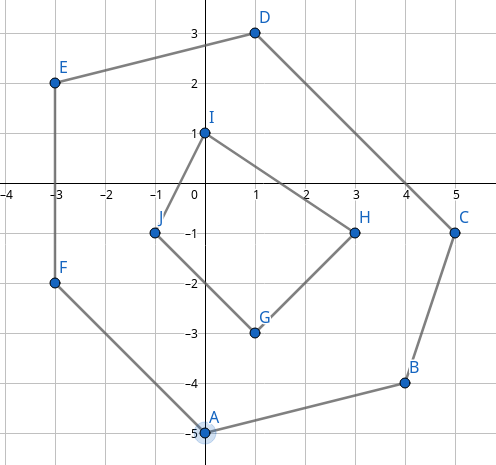
\includegraphics[scale=0.4]{./figs/test04.png}
	\caption{Konveksni ovojnici četrtega testnega primera}
	\label{fig:test04}
\end{figure}

\section{Problem 2}

Algoritem za iskanje Delaunay triangulacije je naključnostni s pričakovanim
izvajanjem $O(n\log n)$.

Algoritem vsako točko doda v trenutno Delaunay triangulacijo. Pri tem se bo v
povprečju dodalo $O(1)$ robov in zgodilo $O(1)$ obratov robov. Če imamo
specifično permutacijo točk, ki ležijo na paraboli $y = x^2$:
\begin{equation*}
	P = \{ (t_1, t_1^2), (t_2, t_2^2), ..., (t_n, t_n^2) \}
\end{equation*}
in velja $ 0 < t_1 < t_2 < ... < t_n$, pomeni da je najbolj leva točka $(t_1,
t_1^2)$ soseda vseh ostalih točk v $P$. Če vstavimo točko $(t_0, t_0^2)$, $0 <
t_0 < t_1$, bomo dodali $n$ novih robov v Delaunay triangulacijo. Iz tega sledi,
da v primeru perumatcije $P = \{ (t_n, t_n^2), ..., (t_1, t_1^2) \}$ algoritem
na vsakem koraku doda $n$ robov, kar da časovno zahtevnost $O(n)$. Ker se to
zgodi za vsako točkoS, je končna časovna zahtevnost algoritma $O(n^2)$.

\section{Problem 3}



\bibliographystyle{plain}
\bibliography{references}

\end{document}